% Options for packages loaded elsewhere
\PassOptionsToPackage{unicode}{hyperref}
\PassOptionsToPackage{hyphens}{url}
\PassOptionsToPackage{dvipsnames,svgnames*,x11names*}{xcolor}
%
\documentclass[
]{memoir}
\usepackage{amsmath,amssymb}
\usepackage{lmodern}
\usepackage{ifxetex,ifluatex}
\ifnum 0\ifxetex 1\fi\ifluatex 1\fi=0 % if pdftex
  \usepackage[T1]{fontenc}
  \usepackage[utf8]{inputenc}
  \usepackage{textcomp} % provide euro and other symbols
\else % if luatex or xetex
  \usepackage{unicode-math}
  \defaultfontfeatures{Scale=MatchLowercase}
  \defaultfontfeatures[\rmfamily]{Ligatures=TeX,Scale=1}
  \setmonofont[]{Inconsolata}
\fi
% Use upquote if available, for straight quotes in verbatim environments
\IfFileExists{upquote.sty}{\usepackage{upquote}}{}
\IfFileExists{microtype.sty}{% use microtype if available
  \usepackage[]{microtype}
  \UseMicrotypeSet[protrusion]{basicmath} % disable protrusion for tt fonts
}{}
\makeatletter
\@ifundefined{KOMAClassName}{% if non-KOMA class
  \IfFileExists{parskip.sty}{%
    \usepackage{parskip}
  }{% else
    \setlength{\parindent}{0pt}
    \setlength{\parskip}{6pt plus 2pt minus 1pt}}
}{% if KOMA class
  \KOMAoptions{parskip=half}}
\makeatother
\usepackage{xcolor}
\IfFileExists{xurl.sty}{\usepackage{xurl}}{} % add URL line breaks if available
\IfFileExists{bookmark.sty}{\usepackage{bookmark}}{\usepackage{hyperref}}
\hypersetup{
  pdftitle={Data Science per psicologi},
  pdfauthor={Corrado Caudek},
  colorlinks=true,
  linkcolor=Maroon,
  filecolor=Maroon,
  citecolor=Blue,
  urlcolor=Blue,
  pdfcreator={LaTeX via pandoc}}
\urlstyle{same} % disable monospaced font for URLs
\usepackage{color}
\usepackage{fancyvrb}
\newcommand{\VerbBar}{|}
\newcommand{\VERB}{\Verb[commandchars=\\\{\}]}
\DefineVerbatimEnvironment{Highlighting}{Verbatim}{commandchars=\\\{\}}
% Add ',fontsize=\small' for more characters per line
\usepackage{framed}
\definecolor{shadecolor}{RGB}{248,248,248}
\newenvironment{Shaded}{\begin{snugshade}}{\end{snugshade}}
\newcommand{\AlertTok}[1]{\textcolor[rgb]{0.94,0.16,0.16}{#1}}
\newcommand{\AnnotationTok}[1]{\textcolor[rgb]{0.56,0.35,0.01}{\textbf{\textit{#1}}}}
\newcommand{\AttributeTok}[1]{\textcolor[rgb]{0.77,0.63,0.00}{#1}}
\newcommand{\BaseNTok}[1]{\textcolor[rgb]{0.00,0.00,0.81}{#1}}
\newcommand{\BuiltInTok}[1]{#1}
\newcommand{\CharTok}[1]{\textcolor[rgb]{0.31,0.60,0.02}{#1}}
\newcommand{\CommentTok}[1]{\textcolor[rgb]{0.56,0.35,0.01}{\textit{#1}}}
\newcommand{\CommentVarTok}[1]{\textcolor[rgb]{0.56,0.35,0.01}{\textbf{\textit{#1}}}}
\newcommand{\ConstantTok}[1]{\textcolor[rgb]{0.00,0.00,0.00}{#1}}
\newcommand{\ControlFlowTok}[1]{\textcolor[rgb]{0.13,0.29,0.53}{\textbf{#1}}}
\newcommand{\DataTypeTok}[1]{\textcolor[rgb]{0.13,0.29,0.53}{#1}}
\newcommand{\DecValTok}[1]{\textcolor[rgb]{0.00,0.00,0.81}{#1}}
\newcommand{\DocumentationTok}[1]{\textcolor[rgb]{0.56,0.35,0.01}{\textbf{\textit{#1}}}}
\newcommand{\ErrorTok}[1]{\textcolor[rgb]{0.64,0.00,0.00}{\textbf{#1}}}
\newcommand{\ExtensionTok}[1]{#1}
\newcommand{\FloatTok}[1]{\textcolor[rgb]{0.00,0.00,0.81}{#1}}
\newcommand{\FunctionTok}[1]{\textcolor[rgb]{0.00,0.00,0.00}{#1}}
\newcommand{\ImportTok}[1]{#1}
\newcommand{\InformationTok}[1]{\textcolor[rgb]{0.56,0.35,0.01}{\textbf{\textit{#1}}}}
\newcommand{\KeywordTok}[1]{\textcolor[rgb]{0.13,0.29,0.53}{\textbf{#1}}}
\newcommand{\NormalTok}[1]{#1}
\newcommand{\OperatorTok}[1]{\textcolor[rgb]{0.81,0.36,0.00}{\textbf{#1}}}
\newcommand{\OtherTok}[1]{\textcolor[rgb]{0.56,0.35,0.01}{#1}}
\newcommand{\PreprocessorTok}[1]{\textcolor[rgb]{0.56,0.35,0.01}{\textit{#1}}}
\newcommand{\RegionMarkerTok}[1]{#1}
\newcommand{\SpecialCharTok}[1]{\textcolor[rgb]{0.00,0.00,0.00}{#1}}
\newcommand{\SpecialStringTok}[1]{\textcolor[rgb]{0.31,0.60,0.02}{#1}}
\newcommand{\StringTok}[1]{\textcolor[rgb]{0.31,0.60,0.02}{#1}}
\newcommand{\VariableTok}[1]{\textcolor[rgb]{0.00,0.00,0.00}{#1}}
\newcommand{\VerbatimStringTok}[1]{\textcolor[rgb]{0.31,0.60,0.02}{#1}}
\newcommand{\WarningTok}[1]{\textcolor[rgb]{0.56,0.35,0.01}{\textbf{\textit{#1}}}}
\usepackage{longtable,booktabs,array}
\usepackage{calc} % for calculating minipage widths
% Correct order of tables after \paragraph or \subparagraph
\usepackage{etoolbox}
\makeatletter
\patchcmd\longtable{\par}{\if@noskipsec\mbox{}\fi\par}{}{}
\makeatother
% Allow footnotes in longtable head/foot
\IfFileExists{footnotehyper.sty}{\usepackage{footnotehyper}}{\usepackage{footnote}}
\makesavenoteenv{longtable}
\usepackage{graphicx}
\makeatletter
\def\maxwidth{\ifdim\Gin@nat@width>\linewidth\linewidth\else\Gin@nat@width\fi}
\def\maxheight{\ifdim\Gin@nat@height>\textheight\textheight\else\Gin@nat@height\fi}
\makeatother
% Scale images if necessary, so that they will not overflow the page
% margins by default, and it is still possible to overwrite the defaults
% using explicit options in \includegraphics[width, height, ...]{}
\setkeys{Gin}{width=\maxwidth,height=\maxheight,keepaspectratio}
% Set default figure placement to htbp
\makeatletter
\def\fps@figure{htbp}
\makeatother
\setlength{\emergencystretch}{3em} % prevent overfull lines
\providecommand{\tightlist}{%
  \setlength{\itemsep}{0pt}\setlength{\parskip}{0pt}}
\setcounter{secnumdepth}{5}
\chapterstyle{bianchi}

\usepackage{amsmath}
\usepackage[italian]{babel} 
\usepackage{lmodern} 
\usepackage{booktabs}
\usepackage{hyperref}
\hypersetup{
  colorlinks=true
}
\usepackage[
  labelfont=bf, 
  font={small, it} 
]{caption} 
\usepackage{upquote} % print correct quotes in verbatim-environments
\usepackage[autostyle, italian=quotes]{csquotes}
\usepackage{xfrac}

\raggedbottom % allow variable (ragged) site heights
\frenchspacing
\setlength\parskip{1.5pt plus 1pt minus 0.5pt}

\DeclareMathOperator{\Var}{Var} % Define variance operator
\DeclareMathOperator{\SD}{SD} % Define sd operator
\DeclareMathOperator{\Cov}{Cov} % Define covariance operator
\DeclareMathOperator{\Corr}{Corr} % Define correlation operator
\DeclareMathOperator{\Me}{Me} % Define mediane operator
\DeclareMathOperator{\Mo}{Mo} % Define mode operator
\DeclareMathOperator{\Bin}{Bin} % Define binomial operator
\DeclareMathOperator{\Cauchy}{Cauchy} % Define Cauchy operator
\DeclareMathOperator{\B}{\mathscr{B}} % Define Bernoulli operator
\newcommand{\R}{\textsf{R}} % Define R programming language symbol
\newcommand{\E}{\mathbb{E}} % Define expected value operator
\newcommand{\Real}{\mathbb{R}} % Define real number operator
\newcommand{\Prob}{\mathscr{P}}
\DeclareMathOperator*{\argmin}{arg\,min} % thin space, limits on side in displays
\DeclareMathOperator*{\argmax}{arg\,max} % thin space, limits on side in displays

\usepackage{microtype}

\ifluatex
  \usepackage{selnolig}  % disable illegal ligatures
\fi
\usepackage[]{natbib}
\bibliographystyle{apalike}

\title{Data Science per psicologi}
\author{Corrado Caudek}
\date{2021-09-13}

\usepackage{amsthm}
\newtheorem{theorem}{Teorema}[chapter]
\newtheorem{lemma}{Lemma}[chapter]
\newtheorem{corollary}{Corollario}[chapter]
\newtheorem{proposition}{Proposizione}[chapter]
\newtheorem{conjecture}{Congettura}[chapter]
\theoremstyle{definition}
\newtheorem{definition}{Definizione}[chapter]
\theoremstyle{definition}
\newtheorem{example}{Esempio}[chapter]
\theoremstyle{definition}
\newtheorem{exercise}{Exercizio}[chapter]
\theoremstyle{definition}
\newtheorem{hypothesis}{Hypothesis}[chapter]
\theoremstyle{remark}
\newtheorem*{remark}{Osservazione}
\newtheorem*{solution}{Soluzione}
\begin{document}
\maketitle

{
\hypersetup{linkcolor=}
\setcounter{tocdepth}{1}
\tableofcontents
}
\newpage

\vspace*{5cm}

\thispagestyle{empty}

\hypertarget{part-inferenza-bayesiana}{%
\part*{Inferenza Bayesiana}\label{part-inferenza-bayesiana}}
\addcontentsline{toc}{part}{Inferenza Bayesiana}

\hypertarget{chapter-intro-bayes-inference}{%
\chapter{Il problema inverso}\label{chapter-intro-bayes-inference}}

La statistica descrittiva si occupa della descrizione, sintesi e presentazione delle informazioni contenute nei dati osservati. Essa spesso rappresenta la fase preliminare di uno studio e un ausilio per l'individuazione di possibili modelli da utilizzare nella successiva fase dell'analisi inferenziale. A differenza della statistica descrittiva, quella inferenziale assume che le osservazioni siano il risultato di un campionamento statistico e il suo obiettivo è ricavare informazioni circa l'intera popolazione a partire dall'osservazione di un suo sottoinsieme.

L'aleatorietà del campione è l'aspetto sostanziale che distingue la statistica inferenziale dalla statistica descrittiva. Nel caso più semplice, il campione statistico è trattato come un insieme di realizzazioni di una variabile casuale assunta a modello del fenomeno oggetto di indagine. La natura del campionamento statistico e la distribuzione di tale variabile casuale determinano il modello statistico. La statistica inferenziale consente di stimare, verificare ipotesi, o effettuare previsioni sul fenomeno in esame.

L'inferenza Bayesiana è un approccio all'inferenza statistica in cui le probabilità non sono interpretate come frequenze, proporzioni o concetti analoghi, ma piuttosto come il grado di fiducia che una singola persona attribuisce al verificarsi di un evento sulla base delle proprie conoscenze e delle informazioni di cui dispone. Come suggerito dal nome stesso, la statistica bayesiana è un approccio all'analisi dei dati e alla stima dei parametri basato sul teorema di Bayes.

\hypertarget{inferenza-statistica-come-un-problema-inverso}{%
\section{Inferenza statistica come un problema inverso}\label{inferenza-statistica-come-un-problema-inverso}}

\begin{itemize}
\item
  L'\emph{inferenza deduttiva} procede in maniera deterministica dai fatti verso le conclusioni. Ad esempio, se dico che tutti gli uomini sono mortali e che Socrate è un uomo, posso concludere deduttivamente che Socrate è mortale.
\item
  L'\emph{inferenza induttiva}, invece, procede dalle osservazioni ai fatti. Se pensiamo ai fatti come a ciò che governa o genera le osservazioni, allora l'induzione è una sorta di inferenza inversa.
\item
  L'\emph{inferenza statistica} è un tipo di inferenza induttiva che è specificamente formulata come un problema inverso.
\end{itemize}

L'inferenza bayesiana è formulata nei termini di un problema inverso che segue la regola di Bayes. Per fissare la notazione, nel seguito \(y\) rappresenterà le variabili osservate, ovvero i dati, e \(\theta\) rappresenterà i parametri incogniti di un modello statistico. Sia \(y\) che \(\theta\) sono concepiti come delle variabili casuali. Con \(x\) verranno invece denotate delle quantità note, come i predittori nel modello di regressione.

\hypertarget{funzioni-di-probabilituxe0}{%
\subsection{Funzioni di probabilità}\label{funzioni-di-probabilituxe0}}

L'inferenza bayesiana utilizza le seguenti distribuzioni di probabilità (o densità di probabilità):

\begin{itemize}
\tightlist
\item
  la \emph{distribuzione a priori} \(p(\theta)\) --- la credenza iniziale riguardo alla credibilità di ciascun valore \(\theta\);
\item
  la \emph{funzione di verosimiglianza} \(p(y \mid \theta)\) --- la credibilità che il ricercatore assegnerebbe ai dati osservati se conoscesse il parametro di interesse \(\theta\);
\item
  la \emph{verosimiglianza marginale} \(p(y)\) --- quanto sono credibili i dati \(y\) alla luce della nostra credenza a priori relativamente a \(\theta\). In termini formali:
\end{itemize}

\[
p(y) = \int_\theta p(y, \theta) d\theta = \int_\theta p(y \mid \theta) p(\theta) d\theta.
\]

\begin{itemize}
\tightlist
\item
  la \emph{distribuzione a posteriori} \(p(\theta \mid y)\) --- la nuova credenza a posteriori relativamente alla credibilità di ciascun valore \(\theta\) alla luce dei dati \(Y = y\).
\end{itemize}

\hypertarget{la-regola-di-bayes}{%
\subsection{La regola di Bayes}\label{la-regola-di-bayes}}

Nel contesto di un modello statistico, la formula di Bayes permette di giungere alla distribuzione a posteriori \(p(\theta \mid y)\) per il parametro di interesse \(\theta\), come indicato dalla seguente catena di equazioni:

\begin{align}
p(\theta \mid y)  &= \displaystyle \frac{p(\theta,y)}{p(y)}
 \ \ \ \ \ \mbox{ [definizione di probabilità condizionata]}
\\
&= \displaystyle \frac{p(y \mid \theta) \, p(\theta)}{p(y)}
 \ \ \ \ \ \mbox{ [legge della probabilità composta]}
\\
&=  \displaystyle \frac{p(y \mid\theta) \, p(\theta)}
                        {\int_{\Theta} p(y,\theta) \, d\theta}
 \ \ \ \ \ \mbox{ [legge della probabilità totale]}
\\
&= \displaystyle \frac{p(y \mid\theta) \, p(\theta)}
                        {\int_{\Theta} p(y \mid\theta) \, p(\theta) \, d\theta}
 \ \ \ \ \ \mbox{ [legge della probabilità composta]}
\\
& \propto \displaystyle p(y \mid\theta) \, p(\theta)
\label{eq:bayesmodel}
\end{align}

La regola di Bayes ``inverte'' la probabilità della distribuzione a posteriori \(p(\theta \mid y)\), esprimendola nei termini della funzione di verosimiglianza \(p(y \mid \theta)\) e della distribuzione a priori \(p(\theta)\). L'ultimo passo è importante per la stima della distribuzione a posteriori mediante i metodi Monte Carlo a catena di Markov, in quanto per questi metodi richiedono soltanto che le funzioni di probabilità siano definite a meno di una costante di proporzionalità. In altri termini, per la maggior parte degli scopi dell'inferenza inversa, è sufficiente calcolare la densità a posteriori non normalizzata, ovvero è possibile ignorare il denominatore bayesiano \(p(y)\). La distribuzione a posteriori non normalizzata, dunque, si riduce al prodotto della varosimiglianza e della distribuzione a priori.

Possiamo dire che la regola di Bayes viene usata per aggiornare le credenze a priori su \(\theta\) (ovvero, la distribuzione a priori) in modo tale da produrre le nuove credenze a posteriori \(p(\theta \mid y)\) che combinano le informazioni fornite dai dati \(y\) con le credenze precedenti. La distribuzione a posteriori riflette dunque l'aggiornamento delle credenze del ricercatore alla luce dei dati.

La \eqref{eq:bayesmodel} rende evidente che, in ottica bayesiana, la quantità di interesse \(\theta\) non è fissata come nell'impostazione frequentista, ma è una variabile casuale la cui distribuzione di probabilità è influenzata sia dalle informazioni a priori sia dai dati a disposizione. In altre parole, nell'approccio bayesiano non esiste un valore vero di \(\theta\), ma vogliamo fornire invece un giudizio di probabilità. Prima delle osservazioni, sulla base delle nostre conoscenze assegniamo a \(\theta\) una distribuzione a priori di probabilità. Dopo le osservazioni, correggiamo il nostro giudizio e assegniamo a \(\theta\) una distribuzione a posteriori di probabilità. La distribuzione a posteriori \(p(\theta \mid y)\) contiene tutta l'informazione riguardante il parametro \(\theta\) e viene utilizzata per produrre indicatori sintetici, per la determinazione di stime puntuali o intervallari, e per la verifica d'ipotesi.

\hypertarget{un-esempio-concreto}{%
\section{Un esempio concreto}\label{un-esempio-concreto}}

L'esempio più semplice di inferenza bayesiana è quello nel quale i dati sono rappresentati da una proporzione. Per questo tipo di dati possiamo adottare il seguente modello statistico

\begin{equation}
y  \sim \mbox{Bin}(n, \theta),
\label{eq:binomialmodel}
\end{equation}

\noindent
laddove \(\theta\) è la probabiltà che una prova Bernoulliana assuma il valore 1 e \(n\) corrisponde al numero di prove Bernoulliane. Questo modello statistico assume che le prove Bernoulliane \(y_i\) che costituiscono il campione \(y\) siano tra loro indipendenti e che ciascuna abbia la stessa probabilità \(\theta \in [0, 1]\) di essere un ``successo'' (valore 1). In altre parole, il modello generatore dei dati ha una funzione di massa di probabilità

\[
p(y \mid \theta)
\ = \
\mbox{Bin}(y \mid n, \theta).
\]

Nei capitoli precedenti è stato mostrato come, sulla base del modello statistico binomiale, sia possibile assegnare una probabilità a ciascun possibile valore \(y \in \{0, 1, \dots, n\}\) \emph{assumendo noto il valore del parametro} \(\theta\). Ma ora abbiamo il \emph{problema inverso}, ovvero quello di fare inferenza su \(\theta\) alla luce dei dati campionari \(y\). In altre parole, riteniamo di conoscere il modello probabilistico che ha generato i dati, ma di tale modello non conosciamo i parametri. Nel caso presente, il modello probabilistico è quello binomiale. Noi vogliamo ottenere informazioni sul valore di \(\theta\) conoscendo il numero osservato \(y\) di successi.

La \eqref{eq:binomialmodel} è un \emph{modello statistico}. Tale modello non spiega perché, in ciascuna realizzazione, \(Y\) assume un particolare valore. Questo modello deve piuttosto essere inteso come un costrutto matematico che ha lo scopo di riflettere alcune proprietà del processo corrispondente ad una sequenza di prove Bernoulliane. In questo senso, è simile al modello di Isaac Newton dei moti planetari che utilizza equazioni differenziali. Le equazioni non sono i pianeti, ma solo descrizioni di come si muovono i pianeti in risposta alle forze gravitazionali. Modelli come quello di Newton ci permettono di prevedere alcuni fenomeni, come il moto dei pianeti, ad esempio. Ma in generale i modelli sono solo delle approssimazioni del fenomeno che vogliono descrivere. Anche il modello di Newton, che produce previsioni estremamente accurate di ciò che possiamo osservare a occhio nudo a proposito del moto dei corpi celesti, è solo un'approssimazione dei modelli del moto e dei fenomeni gravitazionali che, in seguito, sono stati introdotti da Albert Einstein. E anche tali modelli successivi sono, a loro volta, solo un caso speciale della più generale teoria della relatività. In altre parole, modelli sempre migliori vengono proposti, laddove ogni successivo modello è migliore di quello precedente in quanto ne migliora le capacità di previsione, è più generale, o è più elegante.

Una parte del lavoro della ricerca in tutte le scienze consiste nel verificare le assunzioni dei modelli e, se necessario, nel migliorare i modelli dei fenomeni considerati. Un modello viene giudicato in relazione al suo obiettivo. Se l'obiettivo del modello molto semplice che stiamo discutendo è quello di prevedere la proporzione di casi nei quali \(y_i = 1\), \(i = 1, \dots, n\), allora un modello con un solo parametro come quello che abbiamo introdotto sopra può essere sufficiente. Ma l'evento \(y_i=1\) (supponiamo: superare l'esame di Psicometria, oppure risultare positivi al COVID-19) dipende da molti fattori e se vogliamo rendere conto di una tale complessità, un modello come quello che stiamo discutendo qui certamente non sarà sufficiente.

Per concludere, un modello è un costrutto matematico il cui scopo è quello di rappresentare un qualche aspetto della realtà. Il valore di un tale strumento dipende dalla sua capacità di ottenere lo scopo per cui è stato costruito.

\hypertarget{notazione}{%
\subsection{Notazione}\label{notazione}}

Per rappresentare in un modo conciso i modelli statistici viene usata una notazione particolare. Ad esempio, invece di scrivere

\[
p(\theta) = \text{Beta}(1, 1),
\]
\noindent
scriviamo:

\[
\theta \sim \text{Beta}(1, 1).
\]

Il simbolo ``\(\sim\)'' viene spesso letto ``è distribuito come''. Possiamo anche pensare che significhi che \(\theta\) costituisce un campione casuale estratto dalla distribuzione Beta(1, 1). Allo stesso modo, per l'esempio presente, la verosimiglianza può essere scritta come:

\[
y \sim \text{Bin}(n, \theta).
\]

\hypertarget{il-problema-inverso}{%
\subsection{Il problema inverso}\label{il-problema-inverso}}

Nel modello statistico che stiamo esaminando, il termine \(n\) viene trattato come una costante nota e \(\theta\) come una \emph{variabile casuale}. Il parametro \(\theta\) del modello rappresenta la probabilità che ciascuna prova Bernoulliana sia un ``successo''. Dato che \(\theta\) è incognito, ma abbiamo a disposione un campione di dati, l'inferenza su \(\theta\) può essere svolta, mediante la regola di Bayes, costruendo la distribuzione a posteriori \(p(\theta \mid y)\). Una volta ottenuta la distribuzione a posteriori possiamo riassumerla, ad esempio, riportando l'intervallo centrale al 95\% della distribuzione di densità, ovvero

\[
\mbox{Pr}\left[ 0.025 \leq \theta \leq 0.975
                \ \Big| \
        Y = y
         \right].
\]

Se vogliamo sapere, per esempio, se la probabilità di \(y_i=1\) sia maggiore di 0.5, possiamo calcolare la probabilità dell'evento

\[
\mbox{Pr}\left[\theta > \frac{1}{2}
                \ \Bigg| \
        Y = y
         \right].
\]

\hypertarget{cosuxe8-un-parametro-del-modello}{%
\subsection{Cos'è un parametro del modello?}\label{cosuxe8-un-parametro-del-modello}}

Il parametro di un modello è un valore che influenza la credibilità dei dati. Ad esempio, il singolo parametro \(\theta\) del modello binomiale determina la forma della funzione di verosimiglianza binomiale. Ricordiamo che, per il modello binomiale, la funzione di verosimiglianza è:

\[ 
p(y \mid \theta, n) = \text{Bin}(y, n, \theta) = \binom{n}{y}\theta^y(1-\theta)^{n-y}. 
\]
Per comprendere il ruolo del parametro \(\theta\), possiamo generare un grafico della verosimiglianza dei dati come funzione di \(\theta\). Poniamo \(y = 23\) e \(n = 30\). La figura mostra, per ogni possibile valore di \(\theta \in [0, 1]\) (sull'asse orizzontale), la verosimiglianza dei dati (sull'asse verticale). Dalla figura notiamo che la credibilità dei dati dipende dal valore del parametro \(\theta\): i dati risultano più o meno verosimili a seconda del valore di \(\theta\).

\begin{figure}

{\centering 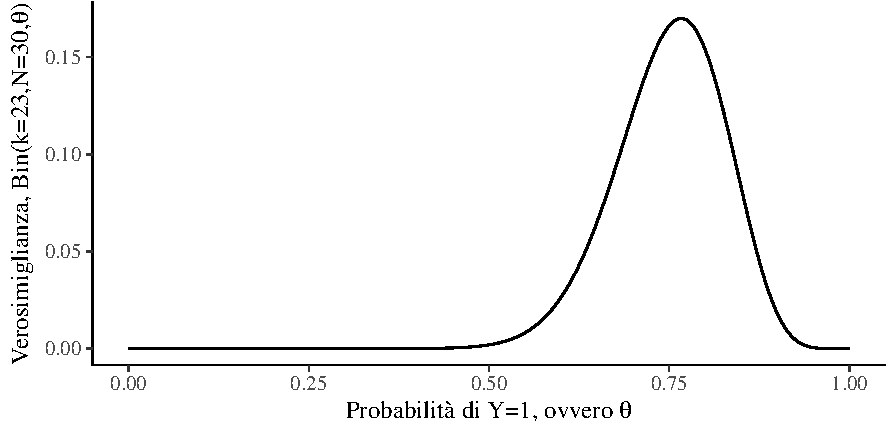
\includegraphics{025_intro_bayes_files/figure-latex/ch-03-02-LH-Binomial-Model-1} 

}

\caption{Funzione di verosimiglianza per il modello binomiale con $y = 23$ e $n = 30$.}\label{fig:ch-03-02-LH-Binomial-Model}
\end{figure}

\hypertarget{la-distribuzione-a-priori-sui-parametri}{%
\subsection{La distribuzione a priori sui parametri}\label{la-distribuzione-a-priori-sui-parametri}}

Quando adottiamo un approccio bayesiano, la distribuzione a priori sui valori dei parametri \(p(\theta)\) è parte integrante del modello statistico. Ciò implica che due modelli bayesiani possono condividere la stessa funzione di verosimiglianza, ma tuttavia devono essere considerati come modelli diversi, se specificano diverse distribuzioni a priori. Ciò significa che, quando diciamo ``Modello binomiale'', intendiamo in realtà un'intera classe di modelli, ovvero tutti i possibili modelli che hanno la stessa verosimiglianza ma diverse distribuzioni a priori su \(\theta\).

Nell'analisi dei dati bayesiana, la distribuzione a priori \(p(\theta)\) codifica le credenze del ricercatore a proposito dei valori dei parametri, prima di avere osservato i dati. Idealmente, le credenze a priori che supportano la specificazione di una distribuzione a priori dovrebbero essere supportate da una qualche motivazione, come ad esempio i risultati di ricerche precedenti, o altre motivazioni giustificabili. Tuttavia, le credenze soggettive sono solo uno dei possibili modi per giustificare le distribuzioni a priori sui parametri.

Possiamo distinguere tre tipi principali di motivazioni per le distribuzioni a priori \(p(\theta)\).

\begin{enumerate}
\def\labelenumi{\arabic{enumi}.}
\tightlist
\item
  Le \emph{distribuzioni a priori soggettive} catturano le credenze del ricercatore nel senso sopra descritto.
\item
  Le \emph{distribuzioni a priori con finalità pratiche} sono distribuzioni a priori che vengono utilizzate pragmaticamente a causa di una loro utilità specifica, ad esempio, perché semplificano un calcolo matematico o una simulazione al computer, o perché aiutano nel ragionamento statistico, come ad esempio quando vengono formulate gli \emph{skeptical priors} che hanno l'obiettivo di lavorare in senso contrario ad una particolare conclusione.
\end{enumerate}

Oltre alla motivazione che giustifica una distribuzione a priori, possiamo distinguere tra diverse distribuzioni a priori in base a quanto fortemente impegnano il ricercatore a ritenere come plausibile un particolare intervallo di valori dei parametri. Il caso più estremo è quello che rivela una totale assenza di conoscenze a priori, il che conduce alle \emph{distribuzioni a priori non informative}, ovvero quelle che assegnano lo stesso livello di credibilità a tutti i valori dei parametri. Le distribuzioni a priori informative, d'altra parte, possono essere \emph{debolmente informative} o \emph{fortemente informative}, a seconda della forza della credenza che esprimono. Il caso più estremo di credenza a priori è quello che riassume il punto di vista del ricercatore nei termini di un \emph{unico valore} del parametro, il che assegna tutta la probabilità (massa o densità) su di un singolo valore di un parametro. Poiché questa non è più una distribuzione di probabilità, sebbene ne soddisfi la definizione, in questo caso si parla di una \emph{distribuzione a priori degenerata}.

La figura seguente mostra esempi di distribuzioni a priori non informative, debolmente o fortemente informative, così come una distribuzione a priori espressa nei termini di un valore puntuale per il modello Binomiale. Le distribuzione a priori illustrate di seguito sono le seguenti:

\begin{itemize}
\tightlist
\item
  \emph{non informativa} : \(\theta_c \sim \text{Beta}(1,1)\);
\item
  \emph{debolmente informativa} : \(\theta_c \sim \text{Beta}(5,2)\);
\item
  \emph{fortemente informativa} : \(\theta_c \sim \text{Beta}(50,20)\);
\item
  \emph{valore puntuale} : \(\theta_c \sim \text{Beta}(\alpha, \beta)\) con \(\alpha, \beta \rightarrow \infty\) e \(\frac{\alpha}{\beta} = \frac{5}{2}\).
\end{itemize}

\begin{figure}

{\centering 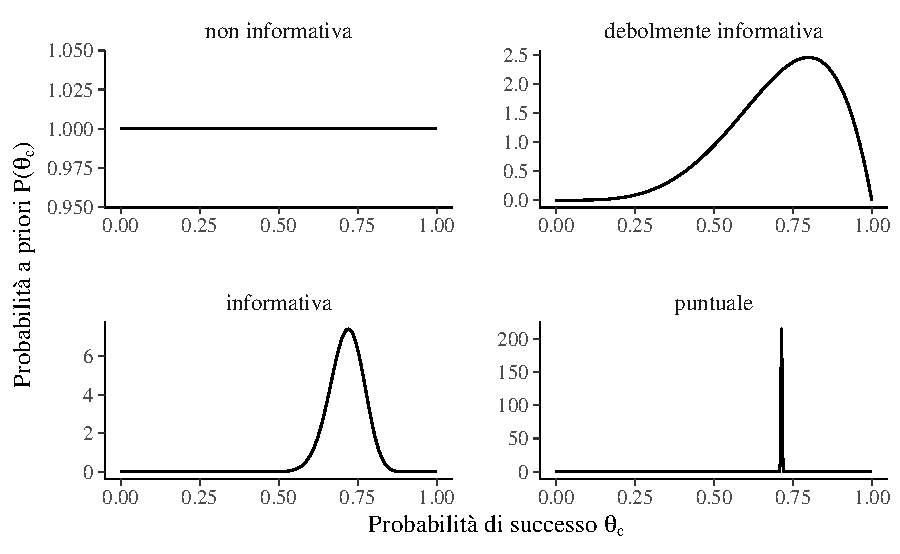
\includegraphics{025_intro_bayes_files/figure-latex/ch-03-02-models-types-of-priors-1} 

}

\caption{Esempi di distribuzioni a priori per il parametro $\theta_c$ nel Modello Binomiale.}\label{fig:ch-03-02-models-types-of-priors}
\end{figure}

\hypertarget{scelta-della-distribuzione-a-priori}{%
\subsection{Scelta della distribuzione a priori}\label{scelta-della-distribuzione-a-priori}}

La selezione delle distribuzioni a priori è stata spesso vista come una delle scelte più importanti che un ricercatore fa quando implementa un modello bayesiano in quanto può avere un impatto sostanziale sui risultati finali. La soggettività delle distribuzioni a priori è evidenziata dai critici come un potenziale svantaggio dei metodi bayesiani. A questa critica, \citet{vandeSchoot2021modelling} rispondono dicendo che, al di là della scelta delle distribuzioni a priori, ci sono molti elementi del processo di inferenza statistica che sono soggettivi, ovvero la scelta del modello statistico e le ipotesi sulla distribuzione degli errori. In secondo luogo, \citet{vandeSchoot2021modelling} notano come le distribuzioni a priori svolgono due importanti ruoli statistici: quello della ``regolarizzazione della stima'', ovvero, il processo che porta ad indebolire l'influenza indebita di osservazioni estreme, e quello del miglioramento dell'efficienza della stima, ovvero, la facilitazione dei processi di calcolo numerico di stima della distribuzione a posteriori.

L'effetto della distribuzione a priori sulla distribuzione a posteriori verrà discusso nel Capitolo \ref{chapter-balance}.

\hypertarget{verosim-marginale}{%
\section{Verosimiglianza marginale}\label{verosim-marginale}}

Al denominatore della regola di Bayes abbiamo la verosimiglianza marginale \(p(y)\). Obiettivo di questo Paragrafo è chiarire questo concetto in riferimento al caso più semplice, ovvero quello della distribuzione binomiale.

Sia \(Y\) una variabile casuale con funzione di massa di probabilità \(p(Y)\). Iniziamo la discussione con un semplice esempio in cui supponiamo che la funzione di massa di probabilità della \(Y\) sia definita nei termini del parametro \(\theta\) e che \(\theta\) possa assumere solo i valori 0.1, 0.5, 0.9, ciascuno con eguale probabilità. In altre parole, la probabilità che \(\theta\) sia 0.1, 0.5, o 0.9 è sempre 1/3.

Ponendo \(n = 30\) e \(y = 23\), ad esempio, la funzione di verosimiglianza diventa

\[
p(y = 23, n = 30 \mid \theta) = \binom{30}{23} \theta^{23} (1-\theta)^{7}.
\]
La \emph{verosimiglianza marginale} \(p(y = 23, n = 30)\) basata su \(\theta\) si ottiene marginalizzando rispetto al parametro \(\theta\): per ogni possibile valore del parametro \(\theta\), calcoliamo il valore della verosimiglianza e lo moltiplichiamo per la probabilità di \(\theta\); poi sommiamo tutti i prodotti ottenuti in questo modo. Matematicamente, ciò significa eseguire l'operazione descritta di seguito.

Nell'esempio abbiamo tre possibili valori \(\theta\) che chiameremo \(\theta_1 = 0.1\), \(\theta_2 = 0.5\) e \(\theta_3 = 0.9\). Ciascuno ha probabilità 1/3, quindi \(p(\theta_1) = p(\theta_2) = p(\theta_3) = 1/3\). Date queste informazioni possiamo calcolare la verosimiglianza marginale come segue:

\begin{align}
p(y = 23, n = 30) &= \binom{30}{23} \theta_1^{23} (1-\theta_1)^{7} \cdot p(\theta_1) \notag\\
&+ \binom{30}{23} \theta_2^{23} (1-\theta_2)^{7} \cdot p(\theta_2) \notag\\
&+ \binom{30}{23} \theta_3^{23} (1-\theta_3)^{7} \cdot p(\theta_3) \notag,
\end{align}

\noindent
ovvero

\begin{align}
p(y = 23, n = 30) &= \binom{30}{23} 0.1^{23} (1-0.1)^{7} \cdot \frac{1}{3} \notag\\
&+ \binom{30}{23} 0.5^{23} (1-0.5)^{7} \cdot \frac{1}{3} \notag\\
&+ \binom{30}{23} 0.9^{23} (1-0.9)^{7} \cdot \frac{1}{3} \notag.
\end{align}

È dunque possibile considerare la verosimiglianza marginale come una sorta di media ponderata della verosimiglianza, nella quale i ``pesi'' dipendono dalla credibilità dei valori del parametro.

L'esempio che abbiamo presentato sopra è artificiale perché al parametro \(\theta\) abbiamo attribuito solo tre possibili valori. In realtà, \(\theta\) può assumere tutti i possibili valori compresi nell'intervallo {[}0, 1{]} e dunque la somma che dobbiamo calcolare avrà infiniti addendi. Dal punto di vista matematico, una tale somma corrisponde all'integrale:

\[
p(y = 23, n = 30) = \int_0^1 \binom{30}{23} \theta^{23} (1-\theta)^{7} d\theta.
\]

\noindent
L'integrale precedente descrive esattamente le stesse operazioni che abbiamo discusso nell'esempio ``artificiale'' in cui \(\theta\) poteva assumere solo tre valori, eccetto che ora dobbiamo eseguire la somma dei prodotti calcolati su tutti gli infiniti valori \(\theta\). Questo integrale corrisponde alla ``marginalizzazione'' del parametro \(\theta\). Non è tuttavia necessario eseguire una tale operazione di maginalizzazione in forma analitica in quanto il precedente integrale può essere calcolato con R:

\begin{Shaded}
\begin{Highlighting}[]
\NormalTok{BinLik }\OtherTok{\textless{}{-}} \ControlFlowTok{function}\NormalTok{(theta) \{}
  \FunctionTok{choose}\NormalTok{(}\DecValTok{30}\NormalTok{, }\DecValTok{23}\NormalTok{) }\SpecialCharTok{*}\NormalTok{ theta}\SpecialCharTok{\^{}}\DecValTok{23} \SpecialCharTok{*}\NormalTok{ (}\DecValTok{1} \SpecialCharTok{{-}}\NormalTok{ theta)}\SpecialCharTok{\^{}}\DecValTok{7}
\NormalTok{\}}
\FunctionTok{integrate}\NormalTok{(BinLik, }\AttributeTok{lower =} \DecValTok{0}\NormalTok{, }\AttributeTok{upper =} \DecValTok{1}\NormalTok{)}\SpecialCharTok{$}\NormalTok{value}
\CommentTok{\#\textgreater{} [1] 0.03225806}
\end{Highlighting}
\end{Shaded}

\hypertarget{soluzione-analitica}{%
\subsection{Soluzione analitica}\label{soluzione-analitica}}

Qui di seguito è riportata la derivazione analitica. Sia \(\theta \sim \Beta(a, b)\) e sia \(y = \{y_1, \dots, y_n\} \sim \Bin(\theta, n)\). Ponendo

\[
B(a, b) = \frac{\Gamma(a)\Gamma(b)}{\Gamma(a+b)},
\]

\noindent
la verosimiglianza marginale diventa

\begin{align}
p(y) &= \binom{n}{y} \int p(y \mid \theta) p(\theta) d\theta \notag\\
&= \binom{n}{y}\int_0^1 \theta^{y} (1 - \theta)^{n- y} \frac{1}{B(a,b)} \theta^{a-1} (1-\theta)^{b-1} d \theta \notag\\
&= \binom{n}{y}\frac{1}{B(a,b)} \int_0^1 \theta^{y + a - 1} (1-\theta)^{n- y + b-1} \notag\\
&= \binom{n}{y}\frac{B(y + a, n- y + b)}{B(a,b)},
\end{align}

\noindent
in quanto

\begin{align}
\int_0^1 \frac{1}{B(a,b)} \theta^{a-1} (1-\theta)^{b-1} d \theta &= 1\notag\\
\frac{1}{B(a,b)} \int_0^1  \theta^{a-1} (1-\theta)^{b-1} d \theta &= 1\notag\\
\int_0^1  \theta^{a-1} (1-\theta)^{b-1} d \theta &= B(a,b). \notag
\end{align}

\noindent
Continuiamo con l'esempio precedente. Per replicare il risultato trovato per via numerica con R, assumiamo una distribuzione a priori uniforme, ovvero \(\Beta(1, 1)\). I valori del problema sono i seguenti:

\begin{Shaded}
\begin{Highlighting}[]
\NormalTok{a }\OtherTok{\textless{}{-}} \DecValTok{1}
\NormalTok{b }\OtherTok{\textless{}{-}} \DecValTok{1}
\NormalTok{y }\OtherTok{\textless{}{-}} \DecValTok{23}
\NormalTok{n }\OtherTok{\textless{}{-}} \DecValTok{30}
\end{Highlighting}
\end{Shaded}

\noindent
e dunque

\begin{Shaded}
\begin{Highlighting}[]
\NormalTok{alpha }\OtherTok{\textless{}{-}}\NormalTok{ y }\SpecialCharTok{+}\NormalTok{ a}
\NormalTok{beta }\OtherTok{\textless{}{-}}\NormalTok{ n }\SpecialCharTok{{-}}\NormalTok{ y }\SpecialCharTok{+}\NormalTok{ b}
\end{Highlighting}
\end{Shaded}

\noindent
Definiamo

\begin{Shaded}
\begin{Highlighting}[]
\NormalTok{B }\OtherTok{\textless{}{-}} \ControlFlowTok{function}\NormalTok{(a, b) \{}
\NormalTok{  (}\FunctionTok{gamma}\NormalTok{(a) }\SpecialCharTok{*} \FunctionTok{gamma}\NormalTok{(b)) }\SpecialCharTok{/} \FunctionTok{gamma}\NormalTok{(a }\SpecialCharTok{+}\NormalTok{ b)}
\NormalTok{\}}
\end{Highlighting}
\end{Shaded}

\noindent
Il risultato cercato si ottiene con

\begin{Shaded}
\begin{Highlighting}[]
\FunctionTok{choose}\NormalTok{(}\DecValTok{30}\NormalTok{, }\DecValTok{23}\NormalTok{) }\SpecialCharTok{*} \FunctionTok{B}\NormalTok{(alpha, beta) }\SpecialCharTok{/} \FunctionTok{B}\NormalTok{(a, b)}
\CommentTok{\#\textgreater{} [1] 0.03225806}
\end{Highlighting}
\end{Shaded}

In conclusione, nel caso di una verosimiglianza binomiale \(y = \sim \Bin(\theta, n)\) e di una distribuzione a priori \(\theta \sim \Beta(a, b)\), la verosimiglianza marginale diventa

\begin{equation}
\binom{n}{y}\frac{B(y + a, n - y + b)}{B(a, b)}.
\label{eq:constant-norm-beta-binom}
\end{equation}

\hypertarget{la-distribuzione-a-posteriori}{%
\section{La distribuzione a posteriori}\label{la-distribuzione-a-posteriori}}

Ci sono due metodi principali per calcolare la distribuzione a posteriori \(p(\theta \mid y)\):

\begin{itemize}
\tightlist
\item
  una precisa derivazione matematica formulata nei termini della distribuzione a priori coniugata alla distribuzione a posteriori (si veda il Capitolo \ref{chapter-distr-coniugate}); tale procedura però ha un'applicabilità molto limitata;
\item
  un metodo approssimato, molto facile da utilizzare in pratica, che dipende da metodi Monte Carlo basati su Catena di Markov (MCMC).
\end{itemize}

Una volta calcolata la distribuzione a posteriori dobbiamo riassumerla in qualche modo. Questo problema verrà discusso nel Capitolo \ref{chapter-sintesi-distr-post}.

\hypertarget{considerazioni-conclusive}{%
\section*{Considerazioni conclusive}\label{considerazioni-conclusive}}
\addcontentsline{toc}{section}{Considerazioni conclusive}

In base all'approccio bayesiano, invece di dire che il parametro di interesse di un modello statistico ha un valore vero ma sconosciuto, diciamo che, prima di eseguire l'esperimento, è possibile assegnare una distribuzione di probabilità, che chiamano stato di credenza, a quello che è il vero valore del parametro. Questa distribuzione a priori può essere nota (per esempio, sappiamo che la distribuzione dei punteggi del QI è normale con media 100 e deviazione standard 15) o può essere del tutto arbitraria. L'inferenza bayesiana procede poi nel modo seguente: si raccolgono alcuni dati e si calcola la probabilità dei possibili valori del parametro \emph{alla luce} dei dati osservati. Questa nuova distribuzione di probabilità è chiamata ``distribuzione a posteriori''. L'approccio bayesiano riassumere l'incertezza dell'inferenza fornendo un intervallo di valori sulla distribuzione di probabilità a posteriori che include il 95\% della probabilità --- questo intervallo è chiamato ``intervallo di credibilità del 95\%''.

\hypertarget{appendix-appendix}{%
\appendix}


\hypertarget{simbologia-di-base}{%
\chapter{Simbologia di base}\label{simbologia-di-base}}

Per una scrittura più sintetica possono essere utilizzati alcuni simboli
matematici.

\begin{itemize}
\item
  L'operatore logico booleano \(\land\) significa ``e'' (congiunzione
  forte) mentre il connettivo di disgiunzione \(\lor\) significa ``o''
  (oppure) (congiunzione debole).
\item
  Il quantificatore esistenziale \(\exists\) vuol dire ``esiste almeno
  un'' e indica l'esistenza di almeno una istanza del concetto/oggetto
  indicato. Il quantificatore esistenziale di unicità \(\exists!\)
  (``esiste soltanto un'') indica l'esistenza di esattamente una istanza
  del concetto/oggetto indicato. Il quantificatore esistenziale
  \(\nexists\) nega l'esistenza del concetto/oggetto indicato.
\item
  Il quantificatore universale \(\forall\) vuol dire ``per ogni.''
\item
  L'implicazione logica ``\(\Rightarrow\)'' significa ``implica'' (se
  \ldots allora). \(P \Rightarrow Q\) vuol dire che \(P\) è condizione
  sufficiente per la verità di \(Q\) e che \(Q\) è condizione necessaria
  per la verità di \(P\).
\item
  L'equivalenza matematica ``\(\iff\)'' significa ``se e solo se'' e indica
  una condizione necessaria e sufficiente, o corrispondenza biunivoca.
\item
  Il simbolo \(\vert\) si legge ``tale che.''
\item
  Il simbolo \(\triangleq\) (o \(:=\)) si legge ``uguale per definizione.''
\item
  Il simbolo \(\Delta\) indica la differenza fra due valori della
  variabile scritta a destra del simbolo.
\item
  Il simbolo \(\propto\) si legge ``proporzionale a.''
\item
  Il simbolo \(\approx\) si legge ``circa.''
\item
  Il simbolo \(\in\) della teoria degli insiemi vuol dire ``appartiene'' e
  indica l'appartenenza di un elemento ad un insieme. Il simbolo
  \(\notin\) vuol dire ``non appartiene.''
\item
  Il simbolo \(\subseteq\) si legge ``è un sottoinsieme di'' (può
  coincidere con l'insieme stesso). Il simbolo \(\subset\) si legge ``è
  un sottoinsieme proprio di.''
\item
  Il simbolo \(\#\) indica la cardinalità di un insieme.
\item
  Il simbolo \(\cap\) indica l'intersezione di due insiemi. Il simbolo
  \(\cup\) indica l'unione di due insiemi.
\item
  Il simbolo \(\emptyset\) indica l'insieme vuoto o evento impossibile.
\item
  In matematica, \(\argmax\) identifica l'insieme dei punti per i quali una data funzione raggiunge il suo massimo. In altre parole, \(\argmax_x f(x)\) è l'insieme dei valori di \(x\) per i quali \(f(x)\) raggiunge il valore più alto.
\end{itemize}

\hypertarget{numeri-binari-interi-razionali-irrazionali-e-reali}{%
\chapter{Numeri binari, interi, razionali, irrazionali e reali}\label{numeri-binari-interi-razionali-irrazionali-e-reali}}

\hypertarget{numeri-binari}{%
\section{Numeri binari}\label{numeri-binari}}

I numeri più semplici sono quelli binari, cioè zero o uno. Useremo spesso
numeri binari per indicare se qualcosa è vero o falso, presente o
assente.

I numeri binari sono molto utili per ottenere facilmente delle statistiche riassuntive in R.Supponiamo di chiedere a 10 studenti ``Ti piacciono i mirtilli?'' Poniamo che le risposte siano le seguenti:

\begin{Shaded}
\begin{Highlighting}[]
\NormalTok{opinion }\OtherTok{\textless{}{-}} \FunctionTok{c}\NormalTok{(}\StringTok{\textquotesingle{}Yes\textquotesingle{}}\NormalTok{,}\StringTok{\textquotesingle{}No\textquotesingle{}}\NormalTok{,}\StringTok{\textquotesingle{}Yes\textquotesingle{}}\NormalTok{,}\StringTok{\textquotesingle{}No\textquotesingle{}}\NormalTok{,}\StringTok{\textquotesingle{}Yes\textquotesingle{}}\NormalTok{,}\StringTok{\textquotesingle{}No\textquotesingle{}}\NormalTok{,}\StringTok{\textquotesingle{}Yes\textquotesingle{}}\NormalTok{,}\StringTok{\textquotesingle{}Yes\textquotesingle{}}\NormalTok{,}\StringTok{\textquotesingle{}Yes\textquotesingle{}}\NormalTok{,}\StringTok{\textquotesingle{}Yes\textquotesingle{}}\NormalTok{)}
\NormalTok{opinion}
\CommentTok{\#\textgreater{}  [1] "Yes" "No"  "Yes" "No"  "Yes" "No"  "Yes" "Yes" "Yes"}
\CommentTok{\#\textgreater{} [10] "Yes"}
\end{Highlighting}
\end{Shaded}

Tali risposte possono essere ricodificate nei termini di valori di
verità, ovvero, vero e falso, generalmente denotati rispettivamente come
1 e 0. In R tale ricodifica può essere effettuata mediante l'operatore
\texttt{==} che è un test per l'uguaglianza e restituisce il valore logico VERO
se i due oggetti valutati sono uguali e FALSO se non lo sono:

\begin{Shaded}
\begin{Highlighting}[]
\NormalTok{opinion }\OtherTok{\textless{}{-}}\NormalTok{ opinion }\SpecialCharTok{==} \StringTok{"Yes"}
\NormalTok{opinion}
\CommentTok{\#\textgreater{}  [1]  TRUE FALSE  TRUE FALSE  TRUE FALSE  TRUE  TRUE  TRUE}
\CommentTok{\#\textgreater{} [10]  TRUE}
\end{Highlighting}
\end{Shaded}

R considera i valori di verità e i numeri binari in modo equivalente, con
TRUE uguale a 1 e FALSE uguale a zero. Di conseguenza, possiamo
effettuare operazioni algebriche sui valori logici VERO e FALSO.
Nell'esempio, possiamo sommare i valori di verità e dividere per 10

\begin{Shaded}
\begin{Highlighting}[]
\FunctionTok{sum}\NormalTok{(opinion) }\SpecialCharTok{/} \FunctionTok{length}\NormalTok{(opinion)}
\CommentTok{\#\textgreater{} [1] 0.7}
\end{Highlighting}
\end{Shaded}

in modo tale da calcolare una propozione, il che ci consente di concludere che 7 risposte su 10 sono positive.

\hypertarget{numeri-interi}{%
\section{Numeri interi}\label{numeri-interi}}

Un numero intero è un numero senza decimali. Si dicono \textbf{naturali} i
numeri che servono a contare, come 1, 2, \ldots{} L'insieme dei numeri
naturali si indica con il simbolo \(\mathbb{N}\). È anche necessario
introdurre i numeri con il segno per poter trattare grandezze negative.
Si ottengono così l'insieme numerico dei numeri interi relativi:
\(\mathbb{Z} = \{0, \pm 1, \pm 2, \dots \}\)

\hypertarget{numeri-razionali}{%
\section{Numeri razionali}\label{numeri-razionali}}

I numeri razionali sono i numeri frazionari \(m/n\), dove \(m, n \in N\),
con \(n \neq 0\). Si ottengono così i numeri razionali:
\(\mathbb{Q} = \{\frac{m}{n} \,\vert\, m, n \in \mathbb{Z}, n \neq 0\}\).
È evidente che \(\mathbb{N} \subseteq \mathbb{Z} \subseteq \mathbb{Q}\).
Anche in questo caso è necessario poter trattare grandezze negative. I
numeri razionali non negativi sono indicati con
\(\mathbb{Q^+} = \{q \in \mathbb{Q} \,\vert\, q \geq 0\}\).

\hypertarget{numeri-irrazionali}{%
\section{Numeri irrazionali}\label{numeri-irrazionali}}

Tuttavia, non tutti i punti di una retta \(r\) possono essere
rappresentati mediante i numeri interi e razionali. È dunque necessario
introdurre un'altra classe di numeri. Si dicono \textbf{irrazionali}, e sono
denotati con \(\mathbb{R}\), i numeri che possono essere scritti come una
frazione \(a / b\), con \(a\) e \(b\) interi e \(b\) diverso da 0. I numeri
irrazionali sono i numeri illimitati e non periodici che quindi non
possono essere espressi sotto forma di frazione. Per esempio,
\(\sqrt{2}\), \(\sqrt{3}\) e \({\displaystyle \pi =3,141592\ldots}\) sono
numeri irrazionali.

\hypertarget{numeri-reali}{%
\section{Numeri reali}\label{numeri-reali}}

I punti della retta \(r\) sono quindi ``di più'' dei numeri razionali. Per
poter rappresentare tutti i punti della retta abbiamo dunque bisogno dei
numeri \textbf{reali}. I numeri reali possono essere positivi, negativi o nulli
e comprendono, come casi particolari, i numeri interi, i numeri
razionali e i numeri irrazionali. Spesso in statisticac il numero dei
decimali indica il grado di precisione della misurazione.

\hypertarget{intervalli}{%
\section{Intervalli}\label{intervalli}}

Un intervallo si dice chiuso se gli estremi sono compresi
nell'intervallo, aperto se gli estremi non sono compresi. Le
caratteristiche degli intervalli sono riportate nella tabella seguente.

\begin{longtable}[]{@{}cll@{}}
\toprule
Intervallo & & \\
\midrule
\endhead
chiuso & \([a, b]\) & \(a \leq x \leq b\) \\
aperto & \((a, b)\) & \(a < x < b\) \\
chiuso a sinistra e aperto a destra & \([a, b)\) & \(a \leq x < b\) \\
aperto a sinistra e chiuso a destra & \((a, b]\) & \(a < x \leq b\) \\
\bottomrule
\end{longtable}

\hypertarget{insiemistica}{%
\chapter{Insiemi}\label{insiemistica}}

Un insieme (o collezione, classe, gruppo, \ldots) è un concetto primitivo,
ovvero è un concetto che già possediamo. Georg Cantor l'ha definito nel
modo seguente:

\begin{quote}
un insieme è una collezione di oggetti, determinati e distinti, della nostra percezione o del nostro pensiero, concepiti come un tutto unico; tali oggetti si dicono elementi dell'insieme.
\end{quote}

Mentre non è rilevante la natura degli oggetti che costituiscono
l'insieme, ciò che importa è distinguere se un dato oggetto appartenga o
meno ad un insieme. Deve essere vera una delle due possibilità: il dato
oggetto è un elemento dell'insieme considerato oppure non è elemento
dell'insieme considerato. Due insiemi \(A\) e \(B\) si dicono uguali se sono
formati dagli stessi elementi, anche se disposti in ordine diverso:
\(A=B\). Due insiemi \(A\) e \(B\) si dicono diversi se non contengono gli
stessi elementi: \(A \neq B\). Ad esempio, i seguenti insiemi sono uguali:
\[\{1, 2, 3\} = \{3, 1, 2\} = \{1, 3, 2\}= \{1, 1, 1, 2, 3, 3, 3\}.\]
Gli insiemi sono denotati da una lettera maiuscola, mentre le lettere
minuscole, di solito, designano gli elementi di un insieme. Per esempio,
un generico insieme \(A\) si indica con
\[A = \{a_1, a_2, \dots, a_n\}, \quad \text{con~} n > 0.\]

La scrittura \(a \in A\) dice che \(a\) è un elemento di \(A\). Per dire che
\(b\) non è un elemento di \(A\) si scrive \(b \notin A.\)

Per quegli insiemi i cui elementi soddisfano una certa proprietà che li
caratterizza, tale proprietà può essere usata per descrivere più
sinteticamente l'insieme:
\[
A = \{x ~\vert~ \text{proprietà posseduta da~} x\},
\]
che si legge come ``\(A\) è l'insieme degli elementi \(x\) per cui è vera la proprietà
indicata.'' Per esempio, per indicare l'insieme \(A\) delle coppie di
numeri reali \((x,y)\) che appartengono alla parabola \(y = x^2 + 1\) si può
scrivere:
\[
A = \{(x,y) ~\vert~ y = x^2 + 1\}.
\]
Dati due insiemi \(A\) e \(B\), diremo che \(A\) è un \emph{sottoinsieme} di \(B\) se
e solo se tutti gli elementi di \(A\) sono anche elementi di \(B\):
\[A \subseteq B \iff (\forall x \in A \Rightarrow x \in B).\] Se esiste
almeno un elemento di \(B\) che non appartiene ad \(A\) allora diremo che
\(A\) è un \emph{sottoinsieme proprio} di \(B\):
\[
A \subset B \iff (A \subseteq B, \exists~ x \in B ~\vert~ x \notin A).
\]
Un altro insieme, detto \emph{insieme delle parti}, o insieme potenza, che si
associa all'insieme \(A\) è l'insieme di tutti i sottoinsiemi di \(A\),
inclusi l'insieme vuoto e \(A\) stesso. Per esempio, per l'insieme
\(A = \{a, b, c\}\), l'insieme delle parti è:
\[
\mathcal{P}(A) = \{
\emptyset, \{a\}, \{b\}, \{c\},
 \{a, b\}, \{a, c\}, \{c, b\},
 \{a, b, c\}
\}.
\]

\hypertarget{operazioni-tra-insiemi}{%
\section{Operazioni tra insiemi}\label{operazioni-tra-insiemi}}

Si definisce \textbf{intersezione} di \(A\) e \(B\) l'insieme \(A \cap B\) di tutti
gli elementi \(x\) che appartengono ad \(A\) e contemporaneamente a \(B\):
\[A \cap B = \{x ~\vert~ x \in A \land x \in B\}.\]

Si definisce \textbf{unione} di \(A\) e \(B\) l'insieme \(A \cup B\) di tutti gli
elementi \(x\) che appartengono ad \(A\) o a \(B\), cioè
\[
A \cup B = \{x ~\vert~ x \in A \lor x \in B\}.
\]

\textbf{Differenza}. Si indica con \(A \setminus B\) l'insieme degli elementi di
\(A\) che non appartengono a \(B\):
\[A \setminus B = \{x ~\vert~ x \in A \land x \notin B\}.\]

\textbf{Insieme complementare}. Nel caso che sia \(B \subseteq A\), l'insieme
differenza \(A \setminus B\) è detto insieme complementare di \(B\) in \(A\) e
si indica con \(B^C\).

Dato un insieme \(S\), una \textbf{partizione} di \(S\) è una collezione di
sottoinsiemi di \(S\), \(S_1, \dots, S_k\), tali che
\[S = S_1 \cup S_2 \cup \dots S_k\] e
\[S_i \cap S_j, \quad \text{con~} i \neq j.\]

La relazione tra unione, intersezione e insieme complementare è data
dalle leggi di DeMorgan: \[(A \cup B)^c = A^c \cap B^c,\]
\[(A \cap B)^c = A^c \cup B^c.\]

\hypertarget{diagrammi-di-eulero-venn}{%
\section{Diagrammi di Eulero-Venn}\label{diagrammi-di-eulero-venn}}

In molte situazioni è utile servirsi dei cosiddetti diagrammi di
Eulero-Venn per rappresentare gli insiemi e verificare le proprietà
delle operazioni tra insiemi (si veda la figura~\ref{fig:sets-venn-diagrams}.
I diagrammi di Venn sono così nominati in onore del matematico inglese del diciannovesimo secolo John Venn anche se Leibnitz e Eulero avevano già in precedenza utilizzato rappresentazioni simili.
In tale rappresentazione, gli insiemi sono individuati da regioni del piano delimitate da una curva chiusa. Nel caso di insiemi finiti, è possibile evidenziare esplicitamente alcuni elementi di un insieme mediante punti, quando si
possono anche evidenziare tutti gli elementi degli insiemi considerati.

\begin{figure}

{\centering 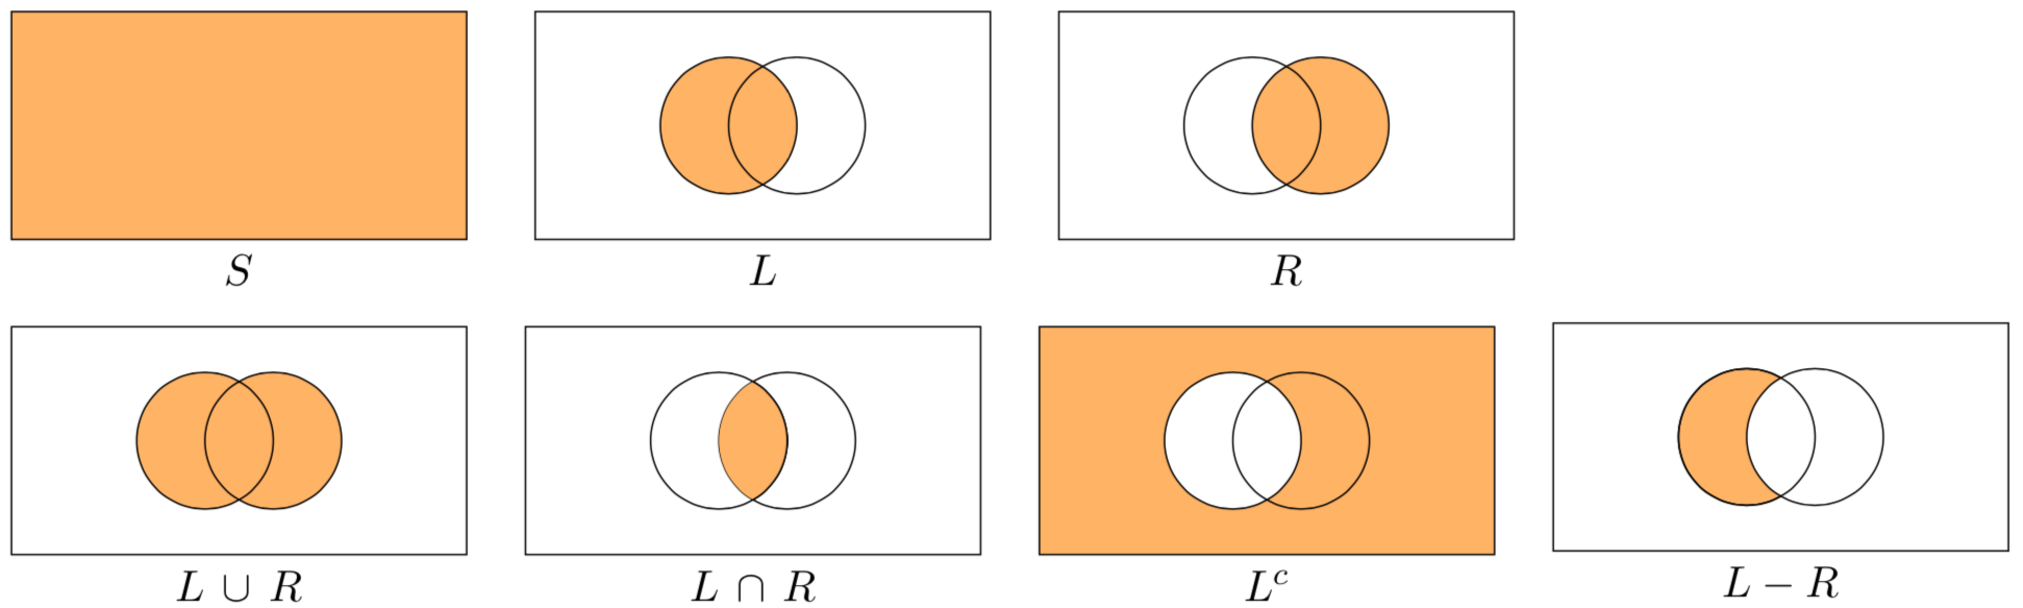
\includegraphics[width=1\linewidth]{images/sets-venn-diagrams} 

}

\caption{In tutte le figure $S$ è la regione delimitata dal rettangolo, $L$ è la regione all'interno del cerchio di sinistra e $R$ è la regione all'interno del cerchio di destra. La regione evidenziata mostra l'insieme indicato sotto ciascuna figura.}\label{fig:sets-venn-diagrams}
\end{figure}

I diagrammi di Eulero-Venn che forniscono una dimostrazione delle leggi
di DeMorgan sono forniti nella figura \ref{fig:demorgan}.

\begin{figure}

{\centering 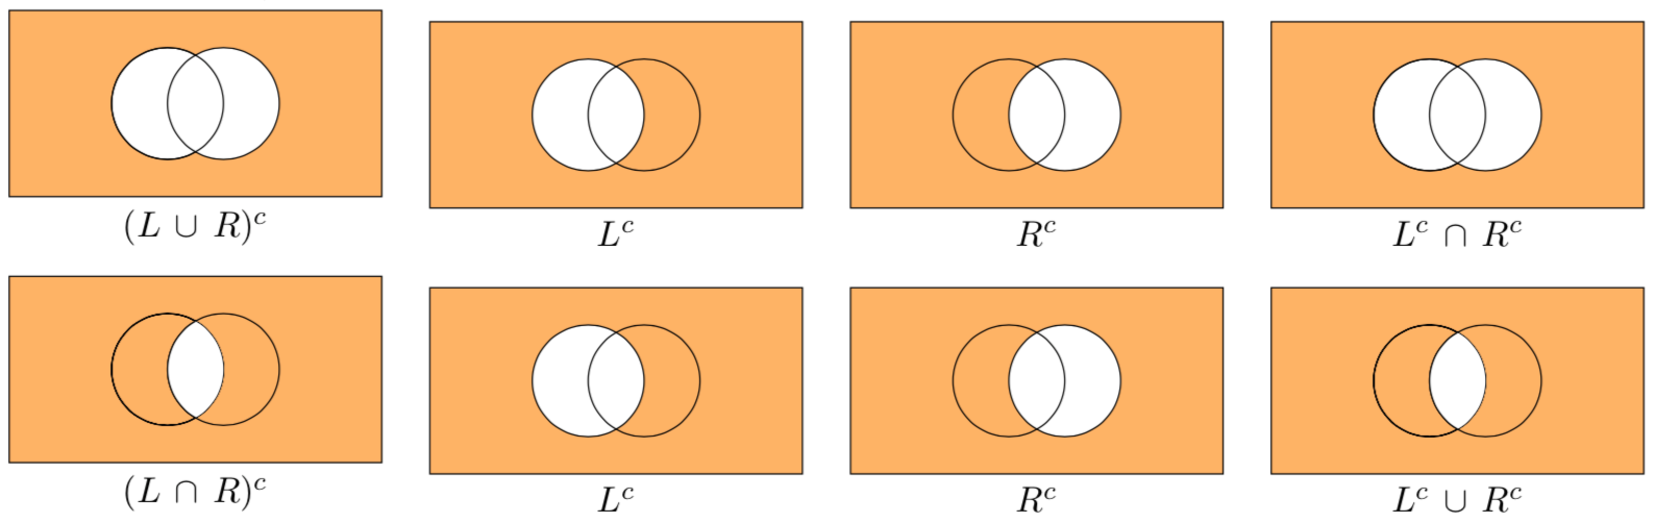
\includegraphics[width=1\linewidth]{images/demorgan} 

}

\caption{Dimostrazione delle leggi di DeMorgan.}\label{fig:demorgan}
\end{figure}

\hypertarget{coppie-ordinate-e-prodotto-cartesiano}{%
\section{Coppie ordinate e prodotto cartesiano}\label{coppie-ordinate-e-prodotto-cartesiano}}

Una coppia ordinata \((x,y)\) è l'insieme i cui elementi sono \(x \in A\) e
\(y \in B\) e nella quale \(x\) è la prima componente (o prima coordinata),
\(y\) la seconda. L'insieme di tutte le coppie ordinate costruite a
partire dagli insiemi \(A\) e \(B\) viene detto \textbf{prodotto cartesiano}:
\[A \times B = \{(x, y) ~\vert~ x \in A \land y \in B\}.\] Ad esempio,
sia \(A = \{1, 2, 3\}\) e \(B = \{a, b\}\). Allora,
\[\{1, 2\} \times \{a, b, c\} = \{(1, a), (1, b), (1, c), (2, a), (2, b), (2, c)\}.\]

\hypertarget{cardinalituxe0}{%
\section{Cardinalità}\label{cardinalituxe0}}

Si definisce \textbf{cardinalità} (o potenza) di un insieme finito il numero
degli elementi dell'insieme. Viene indicata con \(\vert A\vert, \#(A)\) o
\(\text{c}(A)\).

\hypertarget{sommatorie}{%
\chapter{Simbolo di somma (sommatorie)}\label{sommatorie}}

Le somme si incontrano costantemente in svariati contesti matematici e statistici quindi abbiamo bisogno di una notazione adeguata che ci consenta di gestirle. La somma dei primi \(n\) numeri interi può essere scritta come \(1+2+\dots+(n-1)+n\), dove `\(\dots\)' ci dice di completare la sequenza definita dai termini che vengono prima e dopo. Ovviamente, una notazione come \(1+7+\dots+73.6\) non avrebbe alcun senso senza qualche altro tipo di precisazione. In generale, nel seguito incontreremo delle somme nella forma
\begin{equation}
x_1+x_2+\dots+x_n,\notag
\end{equation}
dove \(x_i\) è un numero che è stato definito altrove. La notazione precedente, che fa uso dei tre puntini di sospensione, è utile in alcuni contesti ma in altri risulta ambigua. Pertanto la notazione di uso corrente è del tipo
\begin{equation}
  \sum_{i=1}^n x_i\notag
\end{equation}
\noindent
e si legge ``sommatoria per \(i\) che va da \(1\) a \(n\) di \(x_i\).'\,' Il simbolo \(\sum\) (lettera sigma maiuscola dell'alfabeto greco) indica l'operazione di somma, il simbolo \(x_i\) indica il generico addendo della sommatoria, le lettere \(1\) ed \(n\) indicano i cosiddetti \emph{estremi della sommatoria}, ovvero l'intervallo (da \(1\) fino a \(n\) estremi inclusi) in cui deve variare l'indice \(i\) allorché si sommano gli addendi \(x_i\).
Solitamente l'estremo inferiore è \(1\) ma potrebbe essere qualsiasi altri numero \(m < n\). Quindi
\[
  \sum_{i=1}^n x_i = x_1 + x_{2} + \dots + x_{n}.
\]
Per esempio, se i valori \(x\) sono \(\{3, 11, 4, 7\}\), si avrà
\[
  \sum_{i=1}^4 x_i = 3+11+4+7 = 25 
\]
laddove \(x_1 = 3\), \(x_2 = 11\), eccetera. La quantità \(x_i\) nella formula precedente si dice l'\emph{argomento} della sommatoria, mentre la variabile \(i\), che prende i valori naturali successivi indicati nel simbolo, si dice \emph{indice} della sommatoria.

La notazione di sommatoria può anche essere fornita nella forma seguente
\begin{equation}
  \sum_{P(i)} x_i\notag
\end{equation}
dove \(P(i)\) è qualsiasi proposizione riguardante \(i\) che può essere vera o falsa. Quando è ovvio che si vogliono sommare tutti i valori di \(n\) osservazioni, la notazione può essere semplificata nel modo seguente: \(\sum_{i} x_i\) oppure \(\sum x_i\). Al posto di \(i\) si possono trovare altre lettere: \(k, j, l, \dots\),.

\hypertarget{manipolazione-di-somme}{%
\section{Manipolazione di somme}\label{manipolazione-di-somme}}

È conveniente utilizzare le seguenti regole per semplificare i calcoli che coinvolgono l'operatore della sommatoria.

\hypertarget{proprietuxe0-1}{%
\subsection{Proprietà 1}\label{proprietuxe0-1}}

La sommatoria di \(n\) valori tutti pari alla stessa costante \(a\) è pari a \(n\) volte la costante stessa:
\[
  \sum_{i=1}^{n} a =  \underbrace{a + a + \dots + a}_{n~\text{volte}} = n a.
  \]

\hypertarget{proprietuxe0-2-proprietuxe0-distributiva}{%
\subsection{Proprietà 2 (proprietà distributiva)}\label{proprietuxe0-2-proprietuxe0-distributiva}}

Nel caso in cui l'argomento contenga una costante, è possibile riscrivere la sommatoria. Ad esempio con
\[
  \sum_{i=1}^{n} a x_i =  a x_1 + a x_2 + \dots + a x_n
  \]
è possibile raccogliere la costante \(a\) e fare \(a(x_1 +x_2 + \dots + x_n)\). Quindi possiamo scrivere
\[
  \sum_{i=1}^{n} a x_i =  a  \sum_{i=1}^{n} x_i.
  \]

\hypertarget{proprietuxe0-3-proprietuxe0-associativa}{%
\subsection{Proprietà 3 (proprietà associativa)}\label{proprietuxe0-3-proprietuxe0-associativa}}

Nel caso in cui
\[
  \sum_{i=1}^{n} (a + x_i) =  (a + x_1) +  (a + x_1) + \dots  (a + x_n)
  \]
si ha che
\[
  \sum_{i=1}^{n} (a + x_i) =  n a + \sum_{i=1}^{n} x_i.
  \]
È dunque chiaro che in generale possiamo scrivere
\[
  \sum_{i=1}^{n} (x_i + y_i) =  \sum_{i=1}^{n} x_i + \sum_{i=1}^{n} y_i.
  \]

\hypertarget{proprietuxe0-4}{%
\subsection{Proprietà 4}\label{proprietuxe0-4}}

Se deve essere eseguita un'operazione algebrica (innalzamento a potenza, logaritmo, ecc.) sull'argomento della sommatoria, allora tale operazione algebrica deve essere eseguita prima della somma. Per esempio,
\[
\sum_{i=1}^{n} x_i^2 = x_1^2 + x_2^2 + \dots + x_n^2 \neq \left(\sum_{i=1}^{n} x_i \right)^2.
\]

\hypertarget{proprietuxe0-5}{%
\subsection{Proprietà 5}\label{proprietuxe0-5}}

Nel caso si voglia calcolare \(\sum_{i=1}^{n} x_i y_i\), il prodotto tra i punteggi appaiati deve essere eseguito prima e la somma dopo:
\[
\sum_{i=1}^{n} x_i y_i = x_1 y_1 + x_2 y_2 + \dots + x_n y_n,
\]
infatti, \(a_1 b_1 + a_2 b_2 \neq (a_1 + a_2)(b_1 + b_2)\).

\hypertarget{doppia-sommatoria}{%
\section{Doppia sommatoria}\label{doppia-sommatoria}}

È possibile incontrare la seguente espressione in cui figurano una doppia sommatoria e un doppio indice:
\[
\sum_{i=1}^{n}\sum_{j=1}^{m} x_{ij}.
\]
La doppia sommatoria comporta che per ogni valore dell'indice esterno, \(i\) da \(1\) ad \(n\), occorre sviluppare la seconda sommatoria per \(j\) da \(1\) ad \(m\). Quindi,
\[
\sum_{i=1}^{3}\sum_{j=4}^{6} x_{ij} = (x_{1, 4} + x_{1, 5} + x_{1, 6}) + (x_{2, 4} + x_{2, 5} + x_{2, 6}) + (x_{3, 4} + x_{3, 5} + x_{3, 6}).
\]

Un caso particolare interessante di doppia sommatoria è il seguente:
\[
\sum_{i=1}^{n}\sum_{j=1}^{n} x_i y_j
\]
Si può osservare che nella sommatoria interna (quella che dipende dall'indice \(j\)), la quantità \(x_i\) è costante, ovvero non dipende dall'indice (che è \(j\)). Allora possiamo estrarre \(x_i\) dall'operatore di sommatoria interna e scrivere
\[
\sum_{i=1}^{n} \left( x_i \sum_{j=1}^{n} y_j \right).
\]
Allo stesso modo si può osservare che nell'argomento della sommatoria esterna la quantità costituita dalla sommatoria in \(j\) non dipende dall'indice \(i\) e quindi questa quantità può essere estratta dalla sommatoria esterna. Si ottiene quindi
\[
\sum_{i=1}^{n}\sum_{j=1}^{n} x_i y_j = \sum_{i=1}^{n} \left( x_i \sum_{j=1}^{n} y_j \right) = \sum_{i=1}^{n}\ x_i \sum_{j=1}^{n} y_j.
\]

\begin{example}
Si verifichi quanto detto sopra nel caso particolare di \(x = \{2, 3, 1\}\) e \(y = \{1, 4, 9\}\), svolgendo prima la doppia sommatoria per poi verificare che quanto così ottenuto sia uguale al prodotto delle due sommatorie.

\begin{align}
\sum_{i=1}^3 \sum_{j=1}^3 x_i y_j &= x_1y_1 + x_1y_2 + x_1y_3 + 
x_2y_1 + x_2y_2 + x_2y_3 + 
x_3y_1 + x_3y_2 + x_3y_3 \notag\\
&= 2 \times (1+4+9) + 3 \times (1+4+9) + 2 \times (1+4+9) = 84,\notag
\end{align}
ovvero
\[
(2 + 3 + 1) \times (1+4+9) = 84.
\]
\end{example}

  \bibliography{refs.bib,book.bib,packages.bib}

\end{document}
